%% ---------------------------------------------------------------------------
%% 13th NSysS 2026 submission.
%% Format: ACM Conference Proceedings (sigconf), per the NSysS 2026 CFP.
%% ---------------------------------------------------------------------------

%% ===========================================================================
%%                        AUTHOR VISIBILITY SWITCH
%%
%%   \blindtrue   -> names HIDDEN.  Use for the NSysS double-blind submission.
%%                   Adds the acmart "anonymous" and "review" options, prints an
%%                   anonymous byline, suppresses the running-head author list,
%%                   and drops the acknowledgments.
%%
%%   \blindfalse  -> names VISIBLE. Use for the camera-ready version.
%%                   Prints the real author block from Author.tex, the
%%                   "Paul et al." running head, and the acknowledgments.
%%
%% Edit the two lines below and nothing else: exactly one must be uncommented.
%% ===========================================================================
\newif\ifblind
\blindtrue      % <-- ACTIVE: anonymous submission
%\blindfalse    % <-- swap to this for camera-ready

\ifblind
  \documentclass[sigconf,anonymous,review]{acmart}
\else
  \documentclass[sigconf]{acmart}
\fi

%% acmart already provides graphicx, amsmath, amssymb, booktabs, url and
%% hyperref. Do not re-load them, and do not alter margins or type sizes.
\usepackage{tikz}
\usetikzlibrary{arrows.meta, positioning, shapes.geometric}

\AtBeginDocument{%
  \providecommand\BibTeX{{Bib\TeX}}}

%% Rights and conference information. These are placeholders; ACM supplies the
%% definitive commands in the rights confirmation email once the paper is
%% accepted.
\setcopyright{acmlicensed}
\copyrightyear{2026}
\acmYear{2026}
\acmDOI{XXXXXXX.XXXXXXX}
\acmConference[NSysS '26]{The 13th International Conference on Next
  Generation Computing, Communication, Systems and Security}{December 17--19,
  2026}{Cox's Bazar, Bangladesh}
\acmISBN{978-1-4503-XXXX-X/2026/12}

%% Insert the submission ID issued by CMT, then uncomment.
%\acmSubmissionID{XXX}

%% ===========================================================================
%% PAGE BUDGET (NSysS limit: 8 pages including figures, tables and references)
%%
%% Figure sizes are fixed and must not be reduced. If the build still runs
%% long, apply these in order; each is independent and reversible.
%%
%%   1. tables/comparison-table.tex -- drop the "Local clinician display"
%%      column (its content is stated in the prose of Section 2).
%%   2. Ethics_Statement.tex -- keep paragraph 1 and the final two sentences
%%      of paragraph 2; delete the middle of paragraph 2.
%%   3. tables/baud-table.tex -- delete the two 9600 bps rows; Section 4.4
%%      only argues the 38400 bps case.
%%   4. Experimental_Results_And_Discussion.tex -- delete the third bold
%%      paragraph of Section 7.3 ("Throughput gains are argued...").
%%   5. Last resort: comment out \begin{figure}[t]
\centering
\resizebox{\columnwidth}{!}{%
% Explicit coordinates throughout. Relative placement plus curved return paths
% was letting the "enqueue record" and "Prev" labels land on top of the IDLE
% box, so every node and label position below is pinned by hand.
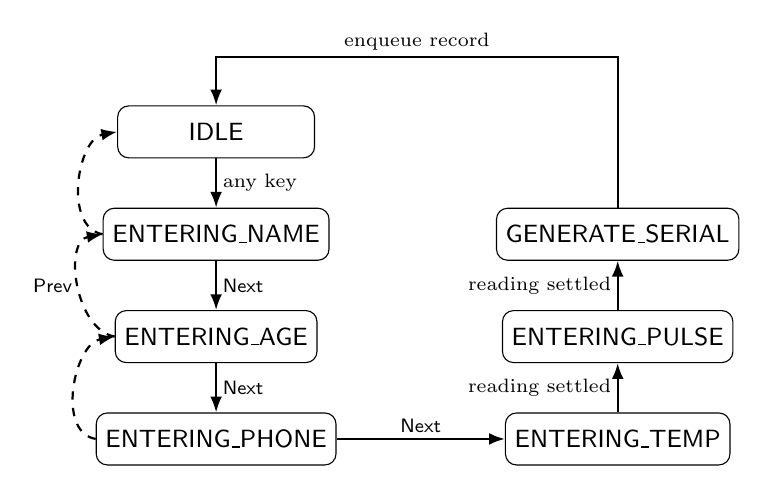
\begin{tikzpicture}[
    st/.style={rectangle, draw, rounded corners, align=center, font=\small,
               minimum width=2.5cm, minimum height=0.66cm},
    lbl/.style={font=\scriptsize, inner sep=2pt},
    ar/.style={-{Latex[length=2mm]}, thick},
    dar/.style={-{Latex[length=2mm]}, thick, dashed}
]

% Forward path. Down the left column, across, then up the right column.
\node[st] (idle)  at (0,0)      {\textsf{IDLE}};
\node[st] (name)  at (0,-1.30)  {\textsf{ENTERING\_NAME}};
\node[st] (age)   at (0,-2.60)  {\textsf{ENTERING\_AGE}};
\node[st] (phone) at (0,-3.90)  {\textsf{ENTERING\_PHONE}};

\node[st] (temp)  at (5.10,-3.90) {\textsf{ENTERING\_TEMP}};
\node[st] (pulse) at (5.10,-2.60) {\textsf{ENTERING\_PULSE}};
\node[st] (gen)   at (5.10,-1.30) {\textsf{GENERATE\_SERIAL}};

\draw[ar] (idle)  -- node[lbl,right]{any key}      (name);
\draw[ar] (name)  -- node[lbl,right]{\textsf{Next}} (age);
\draw[ar] (age)   -- node[lbl,right]{\textsf{Next}} (phone);
\draw[ar] (phone) -- node[lbl,above]{\textsf{Next}} (temp);

% Right-column labels sit in the gap between the columns, clear of the
% horizontal Next arrow at y = -3.90.
\draw[ar] (temp)  -- node[lbl,left]{reading settled} (pulse);
\draw[ar] (pulse) -- node[lbl,left]{reading settled} (gen);

% Return path, routed well above the top row so nothing overlaps.
\draw[ar] (gen.north) -- (5.10,0.95) --
      node[lbl,above,pos=0.5]{enqueue record} (0,0.95) -- (idle.north);

% Prev corrections, drawn as short arcs to the left of the left column.
\draw[dar] (name.west)  to[out=170,in=190] (idle.west);
\draw[dar] (age.west)   to[out=170,in=190]
      node[lbl,left,pos=0.5]{\textsf{Prev}} (name.west);
\draw[dar] (phone.west) to[out=170,in=190] (age.west);

\end{tikzpicture}%
}
\caption{Patient-side registration state machine. Solid arrows are forward
  transitions and dashed arrows are \textsf{Prev} corrections.
  \textsf{GENERATE\_SERIAL} is the only state that enqueues, so a partial
  record can never enter the queue.}
\Description{A state diagram with seven boxes in two columns. The left column
reads from top to bottom: IDLE, ENTERING underscore NAME, ENTERING underscore
AGE, ENTERING underscore PHONE. An arrow labelled any key runs from IDLE down to
ENTERING NAME, and two further arrows labelled Next continue down the column. A
horizontal arrow labelled Next crosses from ENTERING PHONE to ENTERING
underscore TEMP at the foot of the right column. The right column then runs
upward, so an arrow labelled reading settled goes from ENTERING TEMP up to ENTERING
underscore PULSE, and a second reading settled arrow continues up to GENERATE
underscore SERIAL at the top of the right column. From there a long arrow
labelled enqueue record runs up, then left across the top of the figure, and
down into IDLE, closing the cycle. Three short dashed arcs on the far left curve
upward from ENTERING PHONE to ENTERING AGE, from ENTERING AGE to ENTERING NAME,
and from ENTERING NAME to IDLE; they are labelled Prev.}
\label{fig:firmware-fsm}
\end{figure}
 in
%%      Software_And_Firmware_Implementation.tex and delete the
%%      "(Fig.~\ref{fig:firmware-fsm})" reference in the sentence above it.
%%
%% If it comes in UNDER 7 pages there is room to restore detail: the clearest
%% candidate is a short paragraph in Section 7.1 separating the three
%% temperature error sources quantitatively.
%% ===========================================================================

\begin{document}

%% The optional argument is the SHORT title used in the running head. It is
%% required here: without it acmart sets the full title in the header, where it
%% overruns the conference string and the two collide on every odd page.
%% Keep it under roughly 45 characters.
\title[Embedded Patient Queue and Vitals Management]{A Low-Cost
  ATmega32-Based Embedded System for Automated Patient Queue and Health Data
  Management in Private Medical Chambers}

%% Under \blindtrue the acmart "anonymous" option suppresses this block and
%% substitutes an anonymous byline, so the same file serves both versions.
%% Author and affiliation block, ACM "acmart" format.
%%
%% While the "anonymous" class option is active this block is suppressed and
%% acmart prints an anonymous byline instead, so nothing here reaches the
%% reviewed PDF. Removing the "anonymous" option restores it for the
%% camera-ready version.

\author{Kawshik Kumar Paul}
\authornote{Corresponding author.}
\affiliation{%
  \institution{Bangladesh University of Engineering and Technology}
  \department{Department of Computer Science and Engineering}
  \city{Dhaka}
  \country{Bangladesh}}
\email{kawshikbuet17@gmail.com}

\author{Mahdi Hasnat Siyam}
\affiliation{%
  \institution{Bangladesh University of Engineering and Technology}
  \department{Department of Computer Science and Engineering}
  \city{Dhaka}
  \country{Bangladesh}}
\email{mahdibuet3@gmail.com}

\author{Khandokar Md. Rahat Hossain}
\affiliation{%
  \institution{Bangladesh University of Engineering and Technology}
  \department{Department of Computer Science and Engineering}
  \city{Dhaka}
  \country{Bangladesh}}
\email{rahat2975134@gmail.com}


%% A \shortauthors with real names would print them in the running head, which
%% would break double-blind review, so it is set only when names are visible.
\ifblind\else
  \renewcommand{\shortauthors}{Paul et al.}
\fi

\begin{abstract}
Small private medical chambers in low-resource settings still order patients by paper
tokens or verbal agreement, and they measure basic vitals inside the consultation room,
where clinician time is scarcest. We present a stand-alone embedded system that moves both
tasks onto a single low-cost microcontroller. Interaction is split across two separate
stations. A patient-side self-service booth takes identifying details and acquires vital
signs, while a doctor-side console shows the current patient's record and advances the
queue on one button press. A single ATmega32 coordinates both stations, driving an LM35
temperature sensor, an XD-58C optical pulse sensor, a $4\times8$ alphanumeric matrix
keypad and two $16\times2$ character LCDs across 23 of its 32 general-purpose I/O lines.
Unlike the IoT-first architectures that dominate prior work on embedded health monitoring,
the system needs no network, no companion smartphone and no host PC, so a connectivity
outage cannot stall a consultation. Bench validation against commercial reference
instruments places temperature readings within $\pm 1^{\circ}$C and resting pulse within
$\pm 3$~BPM, with button-to-display latency below 1.2~s and queue ordering preserved under
sustained cycling. We also report the clock constraint that shaped the design. At the
factory 1~MHz clock the baud generator cannot reach 38400~bps within the datasheet's error
tolerance, and fuse-selecting the internal 8~MHz oscillator brings the error down to
$0.16\%$.

\end{abstract}

%% CCS concepts. The \ccsdesc lines below are what appear in the PDF. Before
%% camera-ready, visit https://dl.acm.org/ccs, select these same concepts, and
%% paste the generated \begin{CCSXML}...\end{CCSXML} block here: it prints
%% nothing and only supplies the numeric ids ACM's metadata pipeline harvests.
\ccsdesc[500]{Computer systems organization~Embedded systems}
\ccsdesc[500]{Applied computing~Health care information systems}
\ccsdesc[300]{Hardware~Sensor applications and deployments}

\keywords{embedded systems, microcontroller, ATmega32, healthcare automation,
  patient queue management, biomedical sensors, offline-first design,
  low-resource settings}

\maketitle

\section{Introduction}
\label{sec:intro}
A large share of outpatient care in South Asia is delivered not in hospitals but in private
medical chambers, which are one- or two-room practices where a single physician sees patients
in sequence, often with one assistant and no clinical information system. Two routine tasks
dominate the overhead. The first is ordering the queue, typically managed with handwritten
tokens, a paper register, or informal agreement among waiting patients. The second is
recording basic vital signs, which usually happens inside the consultation room after the
patient sits down, so it consumes the one resource the chamber has least of. Measurements of
consultation length in Bangladeshi district and upazila hospitals put the average encounter
at roughly nine minutes~\cite{das2021appointment}, and every minute a thermometer reading and
a pulse count consume within that window is a minute not spent on history taking.

Both tasks are mechanical, and both are amenable to automation. The question is what to automate them
with. The dominant answer in the literature is a networked one. Instrument the patient, stream
readings to a cloud dashboard, and let clinicians reach them through a web or mobile front
end~\cite{irjet2020,rath2021,hrtemp2019}. That approach suits hospitals, and it aligns with the
interoperability goals of the WHO global digital health strategy~\cite{who2021digital}. It is a poor
fit for a two-room chamber, because it adds recurring connectivity cost, makes a consultation depend
on an uplink that may be intermittent, and introduces a failure class the chamber staff cannot
diagnose. That infrastructure assumptions imported from well-resourced settings tend not to survive
contact with developing-region deployments is by now a familiar argument~\cite{brewer2005case}, and a
queue that stalls because a Wi-Fi link dropped is worse than a queue managed on paper.

The complementary work on embedded queue and token systems is offline by construction but scoped to a
different problem. Those systems arbitrate service order at bank counters and ticket windows,
sometimes adding infrastructure such as a GSM link~\cite{qgsm2013} and otherwise confining themselves
to issuing a token number~\cite{eqc2022,arpn2019}. None captures clinical data.

This paper takes the position that the two functions belong in the same device. We present a
stand-alone system, built on one ATmega32 8-bit microcontroller, that guides a patient through
self-registration, acquires body temperature and pulse rate before the patient enters the
consultation room, assigns a queue position, and presents the record to the physician on a
console advanced by a single button. Four requirements shaped it.

\textbf{R1, no network dependency.} Registration, queueing and display must complete with no
uplink, host PC or companion smartphone. \textbf{R2, bounded response.} The physician's control
action must produce a visible result quickly and repeatably. \textbf{R3, operable by
non-technical users.} A first-time patient must register from on-screen prompts alone.
\textbf{R4, commodity parts.} Every component must be locally available at a price a
single-physician practice can justify.

R1 and R4 push toward an 8-bit microcontroller rather than an application processor, and that is what
makes the engineering non-trivial. The ATmega32 offers 32 general-purpose I/O lines, 2~KB of SRAM, and
one 10-bit ADC multiplexed across eight channels~\cite{microchip2020}. From that budget the system
must scan a 32-key matrix, drive two character displays, sample two analog sensors and poll a control
button.

We contribute a complete embedded design integrating FCFS queue arbitration, guided self-registration
with free-text name entry and pre-consultation vital acquisition on one ATmega32, with the full I/O
and memory allocation reported (Sections~\ref{sec:hardware}--\ref{sec:firmware}); a dual-corner
architecture separating patient-side input and sensing from doctor-side review and dequeue control
(Section~\ref{sec:architecture}); the clock constraint we resolved to keep a future serial uplink
viable (Section~\ref{sec:calibration}); and a bench evaluation with an explicit statement of its
limits (Section~\ref{sec:results}).


\section{Related Work}
\label{sec:related}
Work adjacent to this system falls into three groups, covering networked health monitoring,
embedded queue management, and low-cost stand-alone vital measurement.
Table~\ref{tab:comparison} positions the present design against a representative sample of
each. The pattern it makes visible is that sensing and queueing have been treated as separate
problems, and that the systems which integrate sensing do so by adding a network.

\begin{table*}[t]
  \caption{Representative prior systems compared against the proposed design.
    ``Network required'' means the normal operating path depends on a Wi-Fi, GSM
    or Internet link, and ``n/r'' marks a property the cited work does not
    report.}
  \label{tab:comparison}
  \footnotesize
  \begin{tabular}{@{}llccccc@{}}
    \toprule
    Work & Platform & Network & Queue & Vital & Patient self- & Local clinician \\
         &          & required & arbitration & sensing & registration & display \\
    \midrule
    Dharmoji et al.~\cite{irjet2020}        & ESP8266 + Arduino        & Yes (Wi-Fi)  & No           & Pulse, temp. & No  & No \\
    Rath et al.~\cite{rath2021}             & Raspberry Pi BSN         & Yes (MQTT/CoAP) & No        & BSN sensors  & No  & No \\
    Talluri et al.~\cite{hrtemp2019}        & Arduino Uno + web app    & Yes (web)    & No           & Pulse, temp. & No  & No \\
    Gummadi Lahari et al.~\cite{eqc2022}    & 8-bit PIC                & No           & FIFO         & No           & No  & Yes (LCD) \\
    Arun and Priyesh~\cite{qgsm2013}        & MCU + GSM module         & Yes (GSM)    & FIFO         & No           & No  & Yes \\
    Chin et al.~\cite{arpn2019}             & Arduino                  & n/r          & Priority     & No           & No  & Yes \\
    \midrule
    \textbf{This work}                      & \textbf{ATmega32}        & \textbf{No}  & \textbf{FCFS} & \textbf{Pulse, temp.} & \textbf{Yes} & \textbf{Yes (dual LCD)} \\
    \bottomrule
  \end{tabular}
\end{table*}


\subsection{Networked Health Monitoring}
The largest group couples edge sensing to a remote back end. Dharmoji et al.~\cite{irjet2020}
pair an ESP8266 with an Arduino to read pulse and temperature and publish them to ThingSpeak,
so readings are viewed through a cloud dashboard rather than at the point of care. Rath et
al.~\cite{rath2021} work at larger scale, proposing a body-sensor-network architecture for
hospital management with real-time monitoring and prescription handling, and evaluating MQTT
against CoAP in NS-3 simulation to choose a transport. Talluri et al.~\cite{hrtemp2019} read
heart rate and body temperature from an Arduino Uno and surface them through a web
application.

The remote-access capability these systems provide is one our design deliberately gives up, and the
trade-off they accept is that the reporting path is also the display path. Rath et al. treat
reliability and latency under hospital-scale traffic as the governing concerns, which is the wrong
framing for a chamber where the physician is three metres from the patient.

\subsection{Embedded Queue and Token Management}
The second group automates service order without clinical sensing. The electronic queue control
system of Gummadi Lahari et al.~\cite{eqc2022} is the closest offline analogue to our queue
component. An 8-bit PIC maintains FIFO order across service counters and drives an LCD showing
counter and token number, entirely in software and with no external infrastructure. Arun and
Priyesh~\cite{qgsm2013} build queue handling around a GSM link, reintroducing a network dependency
and a per-message cost. Chin et al.~\cite{arpn2019} address a different limitation, that strict FIFO
ignores patients who should be prioritised, and propose an Arduino-based manager that automatically
advances handicapped persons.

All three show that queue arbitration is comfortably within reach of an 8-bit part. None forms a
patient record or captures a physiological measurement, so a chamber deploying any of them would
still take vitals during the consultation. The priority mechanism of Chin et al. is a capability our
strict-FCFS design lacks, and Section~\ref{sec:limitations} returns to it.

\subsection{Stand-Alone Vital Measurement}
The third group establishes that useful vital acquisition is achievable with inexpensive analog
parts. The LM35 is the conventional choice for body temperature because its output is linear at
10~mV/$^{\circ}$C and needs no linearisation or external conditioning before reaching a
microcontroller ADC~\cite{ti2022}. Optical pulse measurement is less forgiving.
Photoplethysmography infers a pulse from light absorbed by perfused tissue, and the waveform is
sensitive to probe placement, contact pressure, perfusion and above all to motion, which produces
artefacts overlapping the signal band that simple filtering cannot remove~\cite{allen2007ppg}. That
sensitivity is intrinsic to the measurement principle rather than to low-cost hardware, it sets the
accuracy ceiling reported in Section~\ref{sec:results}, and it is why the patient-side workflow
enforces a settling period. Expectations should be calibrated accordingly, since clinical electronic
thermometers are held to laboratory accuracy limits measured in tenths of a
degree~\cite{iso80601}, several times tighter than an uncalibrated LM35 and a 10-bit ADC deliver.

The gap this work addresses is integration rather than any individual capability. Queue
arbitration, guided data entry and vital acquisition have each been demonstrated on comparable
hardware. What has not is all three composed into one offline workflow on a single 8-bit
microcontroller, with the two interfaces separated so registration and consultation proceed
concurrently.


\section{System Architecture}
\label{sec:architecture}
% Compact TikZ block diagram of the dual-corner architecture.
\begin{figure*}[t]
\centering
\resizebox{0.92\textwidth}{!}{%
\begin{tikzpicture}[
    node distance=1cm and 1.3cm,
    box/.style={rectangle, draw, rounded corners, minimum width=2.6cm,
                minimum height=0.8cm, align=center},
    group/.style={rectangle, draw, rounded corners, inner sep=5pt},
    arrow/.style={-{Latex[length=3mm]}, thick}
]

% Patient corner group (2x2 layout to save vertical space)
\node[group, label=above:{\textbf{Patient's Corner}}] (patientgroup) {
    \begin{tikzpicture}[node distance=0.4cm and 0.4cm]
        \node[box] (keypad) {$4\times8$ Alphanumeric\\Keypad};
        \node[box, right=of keypad] (temp) {LM35 Temp.\\Sensor};
        \node[box, below=of keypad] (pulse) {XD-58C\\Pulse Sensor};
        \node[box, right=of pulse] (plcd) {$16\times2$ LCD\\(4-bit parallel)};
    \end{tikzpicture}
};

% MCU
\node[box, right=3.4cm of patientgroup] (mcu)
     {ATmega32\\8~MHz internal RC\\(queue, ADC, UART)};

% Doctor corner group
\node[group, right=3.2cm of mcu, label=above:{\textbf{Doctor's Corner}}] (doctorgroup) {
    \begin{tikzpicture}[node distance=0.4cm]
        \node[box] (dlcd) {$16\times2$ LCD\\(I\textsuperscript{2}C)};
        \node[box, below=of dlcd] (btn) {Call-Next Button};
    \end{tikzpicture}
};

% Arrows
\draw[arrow] (patientgroup.east) --
      node[above, yshift=2pt, align=center]{Fields \&\\sensor samples}
      (mcu.west);
\draw[arrow] (mcu.east) --
      node[above, yshift=2pt, align=center]{Dequeued\\record}
      (doctorgroup.west);
\draw[arrow] (doctorgroup.south west) to[bend left=10]
      node[below, yshift=-2pt]{Dequeue} (mcu.south east);

% Optional wireless extension (not used by the delivered firmware)
\node[box, below=0.9cm of mcu] (bt) {Optional HC-05 / UART\\(future work)};
\draw[arrow, dashed] (mcu.south) -- (bt.north);

\end{tikzpicture}%
}
\caption{Dual-corner architecture. One ATmega32 mediates between the patient's
  corner (data entry and sensing) and the doctor's corner (review and queue
  advancement), so the queue is a single in-memory structure with one writer. The
  dashed UART path is wired out but unused.}
\Description{A block diagram with three groups arranged left to right. The left
group, labelled Patient's Corner, is a box containing four smaller boxes in a two
by two arrangement, holding a four by eight alphanumeric keypad, an LM35 temperature
sensor, an XD-58C pulse sensor, and a sixteen by two LCD in four-bit parallel
mode. A thick arrow labelled fields and sensor samples runs right from this group
to a central box labelled ATmega32, eight megahertz internal RC, queue, ADC and
UART. From the ATmega32 a thick arrow labelled dequeued record runs right to the
third group, labelled Doctor's Corner, which contains a sixteen by two I2C LCD
and a call-next button. A return arrow labelled dequeue curves back from the
Doctor's Corner to the ATmega32. Below the ATmega32, a dashed arrow points down
to a box labelled optional HC-05 slash UART, future work.}
\label{fig:system-architecture-block-diagram}
\end{figure*}


The system is organised as two interaction zones coordinated by one microcontroller
(Fig.~\ref{fig:system-architecture-block-diagram}). It is worth stating precisely what is
separated. The corners are distinct at the level of the user interface, since each has its own
display, input device and workflow, and neither can observe the other's intermediate state. They
are not separated at the level of computation, because a single ATmega32 scans the patient-side
keypad, samples both sensors, maintains the queue, polls the doctor's button and refreshes both
displays.

Consolidating onto one controller costs some independence and buys three things under R1 and R4. It
removes the need for an inter-controller link and its failure modes, it halves the controller bill of
materials, and, most importantly, it makes the queue a single in-memory structure with one writer. No
distributed-state problem remains to solve, since a record enqueued by the patient-side workflow is
immediately visible to the doctor-side workflow.

\subsection{Patient's Corner}
The patient interface is a self-service booth built from four peripherals. A $4\times8$ matrix
keypad, assembled from two commodity $4\times4$ membrane keypads, takes the name, age and mobile
number. An LM35 supplies temperature and an XD-58C optical sensor supplies pulse rate. A
$16\times2$ LCD in 4-bit parallel mode carries the prompts and the assigned serial number.

Registration is a strictly sequential dialogue, and the sequencing is what makes R3 achievable. The
LCD requests exactly one field at a time; the firmware will not advance until that field is accepted,
and will not accept a sensor reading until it has settled. A patient therefore never has to decide
what to do next, and cannot submit a record with a missing field. Only after every field is captured
does the firmware assign a serial number and enqueue the record, displaying the number last so the
patient leaves with a position they can reason about while waiting.

Placing the sensors in the booth rather than on the physician's desk is what recovers consultation
time. Temperature and pulse are acquired while the previous patient is still being seen, so
acquisition latency is hidden behind the consultation it would otherwise have extended, and
registration of later patients continues throughout.

\subsection{Doctor's Corner}
The physician's console is deliberately austere. It holds a $16\times2$ LCD on an
I\textsuperscript{2}C backpack, showing the current patient's serial number, name, age,
temperature and pulse, together with one momentary push button that calls the next patient.
There is no menu, no mode and no second control. A press either brings the patient at the head
of the queue onto the display or, once that patient has been seen, releases them and promotes
the next. If the queue is empty the display says so. The physician reads the serial number and calls
that patient in, already holding their vitals on screen. Reducing the console to one degree of freedom
answers R2 directly, leaving no navigation state to remember between patients and no way to reach an
unexpected screen mid-consultation.

Moving this display onto the I\textsuperscript{2}C bus is a necessity rather than a preference.
A second parallel LCD would consume six more I/O lines, and as Section~\ref{sec:hardware} shows,
the pin budget cannot absorb that once the 32-key matrix and two analog channels are accounted
for.

\begin{figure*}[t]
    \centering
    \includegraphics[width=\textwidth]{images/complete-hardware-architecture.png}
    \caption{Proteus schematic of the complete hardware architecture. The
      doctor-side I\textsuperscript{2}C LCD sits on PC0--PC1 and the
      patient-side 4-bit LCD on PD2--PD7, the LM35 and pulse sensor occupy
      ADC0 and ADC1, and the $4\times8$ keypad is driven from port B with row
      sensing on PA4--PA7.}
    \Description{A circuit schematic. At the left are a heart beat sensor module
    and an LM35 temperature sensor, whose analog outputs run to the ADC0 and ADC1
    pins of a central ATmega32 integrated circuit symbol. A pull-up resistor and
    a momentary push button connect to another port A pin. To the upper right of
    the microcontroller, a two-line I2C LCD module connects by just two wires
    labelled SCL and SDA; further right, a separate four-bit parallel LCD module
    connects by six wires from port D. Across the lower half of the figure is a
    grid of thirty-two push-button switches arranged in four rows and eight
    columns, labelled with digit-and-letter pairs such as 1/A and 2/B plus
    dedicated keys for CapsLock, NumLock, Space, BackSpace, Prev and Next. The
    eight column lines run to port B of the microcontroller and the four row
    lines run to port A through four ten-kilohm pull-down resistors.}
    \label{fig:proteus-complete}
\end{figure*}


Fig.~\ref{fig:proteus-complete} gives the schematic-level realisation, captured from the Proteus model
used for pre-deployment verification. It makes the shared-I/O structure concrete, showing the keypad
column drivers on port B, the row sense lines and both ADC inputs on port A, the
I\textsuperscript{2}C pair on port C, and the parallel LCD on port D.


\section{Hardware Implementation}
\label{sec:hardware}
\subsection{Microcontroller Selection}
Four properties of the ATmega32 map onto the requirements of Section~\ref{sec:intro}. Its 10-bit ADC
is multiplexed across eight channels, removing the need for an external converter. Its 32
general-purpose I/O lines are enough, but only just, to host a 32-key matrix alongside two displays
and a control button. Its hardware TWI peripheral is what lets the doctor-side display leave the
parallel bus. And it runs from a factory-calibrated internal RC oscillator, so no crystal is
required~\cite{microchip2020}.

\subsection{I/O and Resource Allocation}
Table~\ref{tab:pinout} gives the complete allocation. Twenty-three of the 32 available lines are in
active use and two more are reserved for the UART, leaving seven free.

\begin{table}[t]
  \caption{ATmega32 I/O allocation: 23 lines active, two reserved, seven free.}
  \label{tab:pinout}
  \small
  \begin{tabular}{@{}llcl@{}}
    \toprule
    Port lines & Function & Lines & Direction \\
    \midrule
    PB0--PB7      & Keypad column drive        & 8 & Output \\
    PA4--PA7      & Keypad row sense           & 4 & Input (pull-down) \\
    PA0 (ADC0)    & LM35 temperature           & 1 & Analog in \\
    PA1 (ADC1)    & XD-58C pulse sensor        & 1 & Analog in \\
    PA2           & Doctor's call button       & 1 & Input (active low) \\
    PC0--PC1      & I\textsuperscript{2}C, doctor LCD & 2 & Bidirectional \\
    PD2--PD7      & Patient LCD, 4-bit parallel & 6 & Output \\
    \midrule
    PD0--PD1      & UART (RXD/TXD), reserved   & 2 & Reserved \\
    PA3, PC2--PC7 & Unallocated                & 7 & n/a \\
    \bottomrule
  \end{tabular}
\end{table}


The keypad dominates the budget, taking twelve lines, more than a third of the total, to drive eight
column outputs and sense four row inputs. That is the price of direct alphanumeric entry, and
Section~\ref{sec:firmware} explains what it buys. Port A is heavily overloaded, carrying both analog
inputs, the four row sense lines and the doctor's button. This is why the keypad driver masks its
direction register rather than writing it wholesale, since an unguarded write to \texttt{DDRA} would
reconfigure the ADC pins mid-acquisition. The display interface asymmetry also pays here. Had the
doctor-side module used the parallel interface rather than an I\textsuperscript{2}C backpack, active
usage would rise from 23 lines to 27, or 29 counting the reserved UART pair, leaving three of 32 free
and no room for an expansion header.

\subsection{Analog Front End}
The LM35 produces 10~mV per degree Celsius with no external circuitry, so its output connects
directly to ADC channel~0~\cite{ti2022}. The XD-58C is an integrated photoplethysmographic module
with on-board amplification and filtering, and its analog output connects to channel~1. The converter
uses the internal 2.56~V bandgap reference, which sets the least significant bit to 2.5~mV and,
against the LM35 transfer function, gives a quantisation step of exactly $0.25^{\circ}$C. AREF is
decoupled to ground through a 1~$\mu$F capacitor as the datasheet specifies~\cite{microchip2020}.

One configuration choice deserves to be flagged rather than defended. The ADC prescaler is left at
its minimum division factor of two, which at 8~MHz yields a 4~MHz conversion clock, whereas the
datasheet specifies 50--200~kHz for full 10-bit accuracy~\cite{microchip2020}. The converter is
therefore clocked well outside the range in which its rated resolution holds. We identify this as a
likely contributor to the temperature spread reported in Section~\ref{sec:results} and as the
cheapest available accuracy improvement, since it costs three bits in one register and no hardware.

\subsection{Clock Configuration and Baud-Rate Error}
\label{sec:calibration}
The internal oscillator ships selected at 1~MHz, and we reconfigured it to 8~MHz through the CKSEL
fuse bits. The reasoning is reproducible from the datasheet, so we set it out here.

\begin{table}[t]
  \caption{UART divisor error at the factory 1~MHz clock versus the fuse-selected
    8~MHz clock. Rows marked $\dagger$ exceed the datasheet's recommended
    $\pm 2.0\%$ receiver error tolerance~\cite{microchip2020}.}
  \label{tab:baud}
  \small
  \begin{tabular}{@{}llcrrr@{}}
    \toprule
    $f_{\mathrm{osc}}$ & Target & U2X & UBRR & Actual & Error \\
    \midrule
    1~MHz & 38400 & 0 & 1  & 31250 & $-18.6\%^{\dagger}$ \\
    1~MHz & 38400 & 1 & 2  & 41667 & $+8.5\%^{\dagger}$ \\
    \midrule
    8~MHz & 38400 & 0 & 12 & 38462 & $+0.16\%$ \\
    8~MHz & 38400 & 1 & 25 & 38462 & $+0.16\%$ \\
    \bottomrule
  \end{tabular}
\end{table}


The ATmega32 derives its UART bit clock by integer division of the system clock. In standard mode the
divisor is $\mathrm{UBRR} = \lfloor f_{\mathrm{osc}}/(16 \times \mathrm{BAUD}) + 0.5 \rfloor - 1$,
with 16 replaced by 8 when the double-speed bit U2X is set~\cite{microchip2020}. Because UBRR is an
integer the achievable rate is quantised, coarsely so when $f_{\mathrm{osc}}$ is low, and the
datasheet's recommended ceiling on receiver error for an 8-bit frame is $\pm 2.0\%$.
Table~\ref{tab:baud} works this through. At 1~MHz, 38400~bps is unreachable, because the nearest
standard-mode divisor yields 31250~bps for an error of $-18.6\%$, roughly nine times the limit, and
double-speed mode improves it only to $+8.5\%$. At 8~MHz the same rate is reachable within
$+0.16\%$ in either mode.

One consequence is worth recording. The internal oscillator is specified to roughly
$\pm 3\%$~\cite{microchip2020}, orders of magnitude looser than the tens of parts per million a quartz
crystal offers. That is adequate for UART framing once the divisor error is this small, but it
propagates into every delay-loop-derived interval in the firmware, including the pulse sampling time
base. The serial path itself is unused by the delivered offline firmware, and establishing that
38400~bps is attainable keeps the optional uplink of Section~\ref{sec:limitations} available without a
hardware revision.


\section{Software and Firmware Implementation}
\label{sec:firmware}
The firmware is embedded C built with AVR-GCC and organised as a cooperative polling superloop with
no interrupt service routines. Each pass tests the keypad, services the active registration state
and tests the doctor's button. We chose this structure for auditability, since with no asynchronous
preemption the worst-case path through the loop can be reasoned about by inspection. The cost is
that every blocking operation, notably ADC acquisition and LCD refresh, extends the loop period for
all other activity, and that is what bounds the latency figures in Section~\ref{sec:results}.

\subsection{Registration State Machine}
The patient-side dialogue is a seven-state machine, shown in Fig.~\ref{fig:firmware-fsm}.
\textsf{IDLE} waits for a first keypress. The three data-entry states each own one field and one
prompt. The two acquisition states drive the LM35 and the pulse sensor and display a countdown so
the patient knows to hold still. \textsf{GENERATE\_SERIAL} allocates the serial number, enqueues the
record and returns to \textsf{IDLE}.

\begin{figure}[t]
\centering
\resizebox{\columnwidth}{!}{%
% Explicit coordinates throughout. Relative placement plus curved return paths
% was letting the "enqueue record" and "Prev" labels land on top of the IDLE
% box, so every node and label position below is pinned by hand.
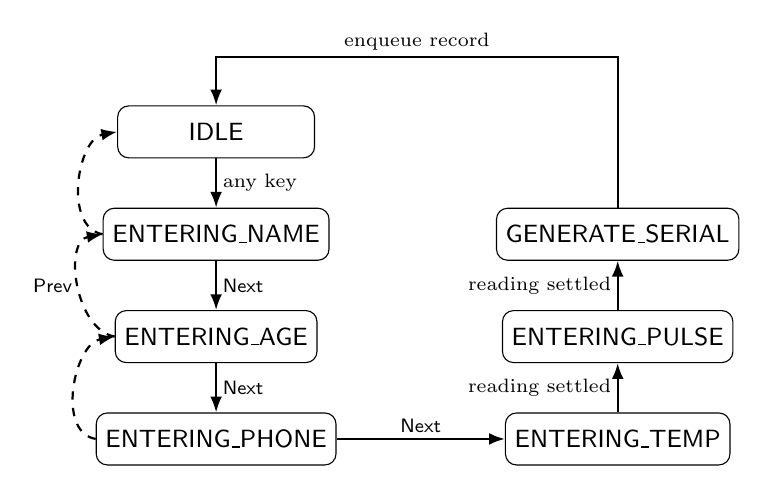
\begin{tikzpicture}[
    st/.style={rectangle, draw, rounded corners, align=center, font=\small,
               minimum width=2.5cm, minimum height=0.66cm},
    lbl/.style={font=\scriptsize, inner sep=2pt},
    ar/.style={-{Latex[length=2mm]}, thick},
    dar/.style={-{Latex[length=2mm]}, thick, dashed}
]

% Forward path. Down the left column, across, then up the right column.
\node[st] (idle)  at (0,0)      {\textsf{IDLE}};
\node[st] (name)  at (0,-1.30)  {\textsf{ENTERING\_NAME}};
\node[st] (age)   at (0,-2.60)  {\textsf{ENTERING\_AGE}};
\node[st] (phone) at (0,-3.90)  {\textsf{ENTERING\_PHONE}};

\node[st] (temp)  at (5.10,-3.90) {\textsf{ENTERING\_TEMP}};
\node[st] (pulse) at (5.10,-2.60) {\textsf{ENTERING\_PULSE}};
\node[st] (gen)   at (5.10,-1.30) {\textsf{GENERATE\_SERIAL}};

\draw[ar] (idle)  -- node[lbl,right]{any key}      (name);
\draw[ar] (name)  -- node[lbl,right]{\textsf{Next}} (age);
\draw[ar] (age)   -- node[lbl,right]{\textsf{Next}} (phone);
\draw[ar] (phone) -- node[lbl,above]{\textsf{Next}} (temp);

% Right-column labels sit in the gap between the columns, clear of the
% horizontal Next arrow at y = -3.90.
\draw[ar] (temp)  -- node[lbl,left]{reading settled} (pulse);
\draw[ar] (pulse) -- node[lbl,left]{reading settled} (gen);

% Return path, routed well above the top row so nothing overlaps.
\draw[ar] (gen.north) -- (5.10,0.95) --
      node[lbl,above,pos=0.5]{enqueue record} (0,0.95) -- (idle.north);

% Prev corrections, drawn as short arcs to the left of the left column.
\draw[dar] (name.west)  to[out=170,in=190] (idle.west);
\draw[dar] (age.west)   to[out=170,in=190]
      node[lbl,left,pos=0.5]{\textsf{Prev}} (name.west);
\draw[dar] (phone.west) to[out=170,in=190] (age.west);

\end{tikzpicture}%
}
\caption{Patient-side registration state machine. Solid arrows are forward
  transitions and dashed arrows are \textsf{Prev} corrections.
  \textsf{GENERATE\_SERIAL} is the only state that enqueues, so a partial
  record can never enter the queue.}
\Description{A state diagram with seven boxes in two columns. The left column
reads from top to bottom: IDLE, ENTERING underscore NAME, ENTERING underscore
AGE, ENTERING underscore PHONE. An arrow labelled any key runs from IDLE down to
ENTERING NAME, and two further arrows labelled Next continue down the column. A
horizontal arrow labelled Next crosses from ENTERING PHONE to ENTERING
underscore TEMP at the foot of the right column. The right column then runs
upward, so an arrow labelled reading settled goes from ENTERING TEMP up to ENTERING
underscore PULSE, and a second reading settled arrow continues up to GENERATE
underscore SERIAL at the top of the right column. From there a long arrow
labelled enqueue record runs up, then left across the top of the figure, and
down into IDLE, closing the cycle. Three short dashed arcs on the far left curve
upward from ENTERING PHONE to ENTERING AGE, from ENTERING AGE to ENTERING NAME,
and from ENTERING NAME to IDLE; they are labelled Prev.}
\label{fig:firmware-fsm}
\end{figure}


Two properties follow from the topology, and both matter for correctness. Enqueueing happens on exactly
one transition, the one out of \textsf{GENERATE\_SERIAL}, which is reachable only after all five
preceding states complete, so a record abandoned halfway cannot reach the queue. That is the
structural guarantee behind the claim that partial records are impossible. Second, the
\textsf{Prev} key provides backward transitions among the data-entry states, letting a mistyped field
be corrected without restarting. The acquisition states offer no backward transition, because a
reading already written into the record is not editable by keypress.

\subsection{Alphanumeric Entry on a $4\times8$ Matrix}
Name entry is the one place a $4\times4$ keypad would have been inadequate, and the reason the design
pays twelve I/O lines for a $4\times8$ matrix. Scanning proceeds in two steps. With all eight columns
driven high, the row nibble identifies which row is asserted, after which each column is pulled low
in turn until the asserted row drops, identifying the column. The result is a key index of
$\mathrm{row} \times 8 + \mathrm{col}$.

Of the 32 keys, 26 carry the letters of the alphabet, four are editing and mode keys (space,
backspace, a caps-lock toggle and an alphabetic/numeric toggle), and two are the \textsf{Prev} and
\textsf{Next} navigation keys handled by the state machine rather than the character layer. The
mapping is direct rather than multi-tap. The first three rows cover A--X at one keypress each and the
fourth supplies Y and Z, so a name costs one press per character with no timing-based disambiguation
to learn. A three-character indicator (\texttt{abc}, \texttt{ABC} or \texttt{123}) in the LCD's
top-right corner keeps the active mode visible, and numeric mode remaps the first three columns to a
telephone-style digit layout. The age and mobile-number fields enter that mode automatically.

Contact bounce is handled in two stages. A detected press is re-tested after 20~ms and discarded if
it has not persisted, after which the scanner is locked out for 100~ms to suppress repeats from a
held key. Fields accumulate into a bounds-checked 16-character buffer, so an over-long entry
saturates rather than overruns.

\subsection{Queue Management}
A simple circular buffer was implemented in C to hold patient records. Each record contains the
assigned serial number; name, age and mobile number as entered at the keypad; the temperature
reading; and the pulse reading in BPM. The record is laid out as fixed-width character fields,
17~bytes each for name, age and mobile number, 10~bytes each for the two readings, and an integer
serial, for 73~bytes per patient. The buffer depth is fixed at compile time, so the static footprint
is $73 \times \mathrm{depth}$ bytes against the 2~KB of SRAM the ATmega32
provides~\cite{microchip2020}. Fixed-width fields make that footprint exactly predictable and
eliminate runtime allocation from the data path.

The enqueue operation is initiated following successful data entry and sensor acquisition. The
doctor's button initiates the dequeue process. Both execute in the same superloop on the same
structure, so there is exactly one writer and no synchronisation is required. The doctor-side control
has two-phase semantics that are not obvious from a single-button interface. The first press after
the queue becomes non-empty promotes the head record onto the console without removing it, so it
stays available for the duration of the consultation, and the next press retires it and promotes its
successor. One button therefore serves both ``show me this patient'' and ``I am done with this
patient''. The button is locked out for 500~ms after each press, and an emptied queue returns the
console to an explicit no-patient message rather than a stale record.

\subsection{Sensor Acquisition and Display}
Both sensors share the single ADC through the input multiplexer. For temperature the raw conversion
is scaled by the LM35 transfer function of 10~mV/$^{\circ}$C~\cite{ti2022} against the 2.56~V
reference, and successive samples are averaged to suppress conversion noise before the result is
committed. For heart rate the pulse waveform is sampled at fixed intervals and excursions above a
threshold are treated as beats, with $\text{BPM} = (60 \times 1000)/T_{\text{beat}}$ where
$T_{\text{beat}}$ is the interval in milliseconds between two consecutive detected peaks. The
acquisition state commits no value until the reading has settled, which is the firmware's response to
the motion sensitivity intrinsic to photoplethysmography~\cite{allen2007ppg}. Because the sampling
interval comes from calibrated delay loops rather than a crystal-driven timer, the time base carries
the $\pm 3\%$ tolerance of the internal RC oscillator, and Section~\ref{sec:results} treats this as
an error source in the reported accuracy.

The patient LCD carries the sequential prompts (``Enter Age'', ``Place Finger on Sensor'') followed by
the serial number, and the doctor LCD is driven over TWI using Fleury's I\textsuperscript{2}C master
library. Both use fixed field widths so a shorter value cannot leave residue from a previous patient
on screen, a real hazard on a display written in place rather than cleared. The firmware was flashed
over ISP with a USBasp programmer, which also set the CKSEL fuse bits, and the design was verified in
the Proteus model of Fig.~\ref{fig:proteus-complete} before assembly.


%% The former standalone "Clock Configuration and Debugging" section is now
%% Section 4.4 inside Hardware Implementation, which is where the constraint
%% belongs and saves a page of the 8-page budget. The \ref{sec:calibration}
%% label moved with it, so all cross-references still resolve.
%The most consequential configuration decision in the build was the system clock, and the
reasoning is reproducible from the datasheet, so we set it out rather than leave it as an
implementation footnote.

The ATmega32 derives its UART bit clock by integer division of the system clock. In
standard mode the divisor register is
$\mathrm{UBRR} = \lfloor f_{\mathrm{osc}} / (16 \times \mathrm{BAUD}) + 0.5 \rfloor - 1$,
with the factor 16 replaced by 8 when the double-speed bit U2X is
set~\cite{microchip2020}. Because UBRR is an integer, the achievable baud rate is
quantised, and the quantisation is coarse when $f_{\mathrm{osc}}$ is low. The datasheet's
recommended ceiling on total receiver error for an 8-bit frame with 16$\times$
oversampling is $\pm 2.0\%$~\cite{microchip2020}.

\begin{table}[t]
  \caption{UART divisor error at the factory 1~MHz clock versus the fuse-selected
    8~MHz clock. Rows marked $\dagger$ exceed the datasheet's recommended
    $\pm 2.0\%$ receiver error tolerance~\cite{microchip2020}.}
  \label{tab:baud}
  \small
  \begin{tabular}{@{}llcrrr@{}}
    \toprule
    $f_{\mathrm{osc}}$ & Target & U2X & UBRR & Actual & Error \\
    \midrule
    1~MHz & 38400 & 0 & 1  & 31250 & $-18.6\%^{\dagger}$ \\
    1~MHz & 38400 & 1 & 2  & 41667 & $+8.5\%^{\dagger}$ \\
    \midrule
    8~MHz & 38400 & 0 & 12 & 38462 & $+0.16\%$ \\
    8~MHz & 38400 & 1 & 25 & 38462 & $+0.16\%$ \\
    \bottomrule
  \end{tabular}
\end{table}


Table~\ref{tab:baud} works the arithmetic through. At the factory-default 1~MHz clock,
38400~bps is simply not reachable: the nearest divisor in standard mode yields 31250~bps,
an error of $-18.6\%$, roughly nine times the recommended limit, and double-speed mode
improves this only to $+8.5\%$, still four times over. The 9600~bps case is salvageable but
only in double-speed mode, standard mode giving $-7.0\%$.

Raising the clock to 8~MHz resolves the problem outright: 38400~bps is then reachable with
an error of $+0.16\%$ in either mode, comfortably inside the ceiling. Reliability was
significantly increased by using the internal 8~MHz oscillator and double-speed UART.

Two aspects of how we got there are worth recording, because both are the kind of
constraint that shapes a low-cost build. The change was made by programming the CKSEL fuse
bits rather than by fitting an external crystal, which was unavailable to us at the time;
fuse programming adds no components and requires no board changes, but a mis-set fuse can
leave the part unable to clock itself and recoverable only through high-voltage
programming, so it is not a reversible experiment. And the internal oscillator that makes
this convenient is specified to roughly $\pm 3\%$~\cite{microchip2020}, an order of
magnitude looser than a crystal: adequate for UART framing once the divisor error is this
small, but propagating into every delay-loop-derived interval in the firmware.

The serial path characterised here is wired out but unused by the delivered firmware, which
operates entirely offline per R1. Establishing that 38400~bps is attainable matters because
it keeps the optional uplink of Section~\ref{sec:limitations} available without a further
hardware revision.


\section{Experimental Results and Discussion}
\label{sec:results}
\begin{table}[t]
  \caption{Observed system performance. Deviations are engineering bounds from
    bench comparison; see Section~\ref{sec:threats} for scope.}
  \label{tab:experimental_results_table}
  \small
  \begin{tabular}{@{}lll@{}}
    \toprule
    Metric & Observation & Reference \\
    \midrule
    Temperature accuracy      & $\pm 1^{\circ}$C, $25$--$40^{\circ}$C & Digital thermometer \\
    Pulse accuracy (resting)  & $\pm 3$ BPM                           & Fingertip oximeter \\
    Button-to-display latency & $< 1.2$ s                             & Direct observation \\
    Queue ordering            & Preserved under cycling               & Enqueue/dequeue cycles \\
    Record footprint          & 73 bytes of 2~KB SRAM                 & Firmware layout \\
    Operating mode            & Offline, stand-alone                  & n/a \\
    \bottomrule
  \end{tabular}
\end{table}


We evaluated the assembled prototype along four axes, covering temperature accuracy, pulse
accuracy, control-path latency and queue robustness under sustained cycling.
Table~\ref{tab:experimental_results_table} summarises the outcomes, and
Section~\ref{sec:threats} states what they do and do not establish. All measurements were taken on
the bench prototype running the delivered offline firmware, with the ATmega32 on its internal
8~MHz oscillator and all peripherals connected as in Section~\ref{sec:hardware}. Sensing accuracy
was assessed against commercial reference instruments rather than laboratory standards, namely a
digital clinical thermometer and a fingertip pulse oximeter, with readings taken from resting
adult volunteers under normal indoor ambient conditions.

\subsection{Sensing Accuracy}
LM35 readings agreed with the reference thermometer to within $\pm 1^{\circ}$C across the range
exercised, approximately $25$--$40^{\circ}$C, which spans room ambient through febrile body
temperature. This is adequate for pre-screening and not adequate for diagnosis, since clinical
electronic thermometers are held to laboratory accuracy limits measured in tenths of a
degree~\cite{iso80601}. Three error sources plausibly account for the spread, and their remedies
differ sharply. Quantisation contributes a hard floor of $0.25^{\circ}$C per LSB, which is small
relative to the observed bound. Uncalibrated sensor tolerance contributes a fixed offset that a
one-point calibration constant in firmware would largely remove. The over-clocked ADC of
Section~\ref{sec:hardware} contributes an unquantified degradation, and of the three it is the
cheapest to fix and the one we would address first.

Pulse readings from the XD-58C agreed with the reference oximeter to within $\pm 3$~BPM under resting
conditions. The dominant source of variation was motion and transient noise during finger placement.
Readings taken immediately on contact were markedly less stable than those taken after a brief
settling period, which is why the acquisition state enforces one. This is characteristic of the
measurement principle rather than of this sensor, since photoplethysmographic amplitude and
morphology vary strongly with probe pressure, perfusion and movement~\cite{allen2007ppg}. A subtler
contributor is the time base. The sampling interval derives from delay loops clocked by the internal
RC oscillator, specified to roughly $\pm 3\%$~\cite{microchip2020}, and a systematic 3\% interval
error maps directly onto the computed rate, about 2~BPM at 70~BPM. A hardware timer with a crystal
reference would remove this term, at the cost of the crystal the design deliberately omits.

\subsection{Control-Path Latency and Queue Robustness}
Responsiveness was measured end to end, from the physical press of the doctor's button to the
appearance of the updated record on the console, so it includes debounce, queue access, string
formatting and the full I\textsuperscript{2}C refresh. Observed latency remained below 1.2~s. Queue
advancement happens once per consultation, so a sub-1.2~s response is imperceptible at that cadence.
The relevant property is not that latency is small but that it is bounded and repeatable, which
follows from the superloop architecture of Section~\ref{sec:firmware}. Note also that the debounce
lockout is a deliberate 500~ms, so roughly half the measured latency is a design constant rather than
computational cost.

Queue integrity was exercised through repeated enqueue and dequeue cycles, checking after each that
records emerged in entry order with none lost or duplicated. Ordering and record integrity held
across sustained cycling, and the two-phase button semantics behaved correctly at the boundaries
that matter in practice. A press against an empty queue produces the no-patient message rather than
a stale or undefined record, and emptying the queue mid-consultation returns the console to that
message rather than leaving the retired patient on screen. The bound here is capacity, not
correctness. With 2~KB of SRAM against a 73-byte record, achievable depth is modest and fixed at
build time, which is not the binding constraint for a waiting room holding a few tens of patients.
For a longer record history, or any requirement to survive a power interruption, the persistent
storage of Section~\ref{sec:limitations} becomes necessary rather than optional.

\subsection{Threats to Validity and Scope}
\label{sec:threats}
The figures above are easy to over-read, so we state their limits explicitly.

\textbf{The sensing results are a bench comparison, not a clinical accuracy study.} Readings were
compared against consumer-grade instruments, themselves uncalibrated against a traceable standard,
on a small group of resting adult volunteers. We therefore report observed deviation bounds rather
than statistical agreement measures such as Bland--Altman limits, which would require a
prespecified population and sample size, and the $\pm 1^{\circ}$C and $\pm 3$~BPM figures are
engineering bounds establishing fitness for triage, not validated accuracy claims. Pulse accuracy
under exertion, in patients with poor peripheral perfusion, or in paediatric and elderly subjects
was not assessed, and photoplethysmography degrades in each case~\cite{allen2007ppg}.

\textbf{No deployment study was conducted.} The claim that a guided sequential dialogue lets a
non-technical patient self-register unaided is a design argument supported by the structure of the
state machine, not a tested result. Completion rate, error rate, time-to-complete and accessibility
for patients with low literacy or impaired vision all remain open, and a field study measuring them
is the most valuable single piece of future work.

\textbf{Throughput gains are argued, not measured.} That booth-side acquisition recovers
consultation time follows from moving acquisition off the physician's critical path, and reported
consultation lengths~\cite{das2021appointment} indicate the magnitude at stake, but we did not
measure consultations with and without the system.


\section{Limitations and Future Work}
\label{sec:limitations}
\textbf{Volatile storage.} The queue resides entirely in SRAM, so a power interruption discards every
waiting record and the chamber falls back to the manual process the system replaced. Where grid supply
is intermittent this is the most serious functional limitation of the current build. The ATmega32
provides 1~KB of internal EEPROM, enough to mirror a working queue of the depth SRAM supports, and
writing each record through on enqueue would make the queue survive a reset with no added components.
An SD card would additionally permit a retained visit history, at the cost of an SPI interface and a
filesystem layer.

\textbf{Strict FCFS ordering.} The queue implements first-come, first-served with no override. This
is the fair default and the behaviour the system was built to enforce, but clinical practice
sometimes requires otherwise, whether for an acutely unwell patient or on the accessibility grounds
motivating the priority scheme of Chin et al.~\cite{arpn2019}. A second console control promoting a
selected record would address this, and any such mechanism must stay visible to waiting patients to
avoid undermining the transparency that motivated automating the queue.

\textbf{Corners tethered by cable.} Both corners wire back to one controller, so their separation is
bounded by cable length and they cannot occupy different rooms as a larger chamber might require.
The reserved UART lines and the 38400~bps operating point established in
Section~\ref{sec:calibration} exist to lift this restriction, since a Bluetooth or Wi-Fi module on
that port would let the console sit in a separate room and would support mobile waiting-list
notification. Any such extension must preserve the property that the offline path keeps working
when the link is down.

\textbf{Accuracy and scale.} Section~\ref{sec:results} identifies three inexpensive corrections, namely
setting the ADC prescaler to bring the conversion clock into the datasheet's 50--200~kHz window,
storing a per-unit calibration offset for the LM35, and deriving the pulse sampling interval from a
hardware timer rather than delay loops. None requires a different microcontroller or sensor. The
architecture also extends to a multi-room variant with one booth feeding several consoles, where the
queue structure generalises directly but the pin budget does not. Placing all consoles on the shared
I\textsuperscript{2}C bus absorbs that growth. Finally, as Section~\ref{sec:threats} notes, guided
self-registration has not been tested with patients, and a deployment study would test the claim this
design rests on most heavily.


\section{Conclusion}
This paper presented a stand-alone embedded system that automates patient queue handling and
pre-consultation vital-sign acquisition for small private medical chambers. The design places
guided self-registration and sensing in a patient-side booth, reduces the physician's interaction
to a single button on a dedicated console, and coordinates both from one ATmega32. It requires no
network, no host PC and no companion device, so no external service sits on the critical path of a
consultation.

The engineering result is that the composition fits. Queue arbitration, free-text alphanumeric
entry over a 32-key matrix, two analog sensor channels and two character displays coexist within 23
of the microcontroller's 32 I/O lines and a 73-byte record against 2~KB of SRAM. Bench validation
placed temperature within $\pm 1^{\circ}$C and resting pulse within $\pm 3$~BPM of commercial
reference instruments, with button-to-display latency below 1.2~s and queue ordering preserved
under sustained cycling. We also documented the clock constraint that shaped the build. At the
factory 1~MHz clock the baud generator cannot reach 38400~bps within the datasheet's error
tolerance, and fuse-selecting the internal 8~MHz oscillator brings the error down to $0.16\%$.

We are equally explicit about what remains unestablished. The sensing figures are engineering bounds
from a bench comparison rather than validated clinical accuracy, the queue does not survive a power
interruption, and guided self-registration has not been tested with patients in a working chamber.
Each is addressable without abandoning the offline, low-cost premise the design rests on, and that
premise is the paper's substantive claim. For a two-room practice, a system which keeps working when
the network does not is worth more than one that reports to the cloud.


\ifblind\else
\begin{acks}
The authors thank Dr.\ A.\ B.\ M.\ Alim Al Islam for supervising this work.
\end{acks}
\fi

\section*{Ethics and Privacy Statement}
The validation reported in Section~\ref{sec:results} was performed on a laboratory bench prototype.
No clinical deployment took place, no patients participated, and no patient records were collected
or retained.

The system nevertheless handles identifying personal data by design. Records live only in volatile
memory, so the device accumulates no persistent identifiable data, and the storage proposed in
Section~\ref{sec:limitations} reverses that property and would need a retention limit and
encryption at rest. Because the console shows a patient's name beside their vitals in plain text,
its placement on the desk is a confidentiality decision as well as an ergonomic one. The absence of
connectivity is itself a privacy benefit, since no data leaves the device, and any wireless
extension should therefore be treated as a change requiring authenticated pairing, encrypted
transport and explicit patient consent. Finally, the temperature and pulse channels are triage
indicators, accurate enough to draw a physician's attention and not accurate enough to support a
clinical decision alone. Misreading that boundary is the most plausible route from this work to
harm, and the system should not be deployed or extended as an autonomous screening device.


\bibliographystyle{ACM-Reference-Format}
\bibliography{References}

\end{document}
